\documentclass[11pt]{article}

\usepackage[a4paper,margin=24mm]{geometry}
\usepackage{kotex}
\usepackage{amsmath}
\usepackage{booktabs}
\usepackage{tabularx}
\usepackage{makecell}
\usepackage{graphicx}
\usepackage{xcolor}
\usepackage{tikz}
\usepackage{pgfplots}
\usepackage[numbers,sort&compress]{natbib}
\usepackage[colorlinks=true,linkcolor=blue!55!black,citecolor=blue!55!black,urlcolor=blue!55!black]{hyperref}

\pgfplotsset{compat=1.17}
\usetikzlibrary{arrows.meta,positioning,shapes.geometric,fit,calc}
\urlstyle{same}

\definecolor{osblue}{HTML}{1F77B4}
\definecolor{osorange}{HTML}{E69F00}
\definecolor{osgreen}{HTML}{009E73}
\definecolor{osred}{HTML}{D55E00}
\definecolor{ospurple}{HTML}{7B3294}
\definecolor{osgray}{HTML}{4D4D4D}

\newcommand{\model}{\texttt{face\_multitask\_v2}}
\newcommand{\detector}{\texttt{Detectorv2}}
\newcommand{\pyfeat}{\texttt{py-feat}}

\title{Py-Feat Detectorv2 기반 실시간 얼굴 행동 분석 웹 데모의\\공개 벤치마크 및 엔드투엔드 성능 분석}
\author{Anonymous Authors}
\date{2026년 7월 22일 초안}

\begin{document}
\maketitle

\begin{abstract}
얼굴 표정, 시선, 자세, 행동 단위(Action Unit, AU)를 실시간으로 추정하는 시스템은 인간 행동 분석, 정서 컴퓨팅, 상호작용형 웹 응용에서 핵심적인 역할을 한다. 본 논문은 Py-Feat \detector{} 기반 Live 웹 데모를 대상으로, 단일 multi-task 모델이 제공하는 얼굴 검출, 478점 mesh, 20개 AU, 7-class emotion, valence/arousal, gaze, 6-DoF pose, 52개 blendshape 출력을 논문 형식으로 정리한다. 성능 평가는 저장소에 원자료와 실행 산출물이 포함되지 않은 점을 고려하여, 공개된 \model{} 모델 카드의 held-out/file-verified 수치, Py-Feat speed-clean-m5max 벤치마크, 그리고 현재 웹 시연 문서의 엔드투엔드 측정치를 엄격히 구분하여 보고한다. 공개 벤치마크에서 배포 체크포인트는 DISFA+ 12-AU macro-F1 0.693, RAF-DB 7-class accuracy 0.910, Aff-Wild2 valence/arousal CCC 0.852/0.799, MPIIGaze 평균 각도 오차 7.05$^\circ$를 보였다. Apple M5 Max MPS 환경에서는 472프레임 비디오 기준 batch 16에서 128.5 FPS를 기록했으며, 웹 데모는 Brave Browser 캡처 기준 약 22.1 FPS와 45 ms 지연시간을 보였다. 본 논문은 이 수치들이 서로 다른 측정 계층, 즉 모델 처리량과 브라우저 포함 엔드투엔드 표시 성능을 나타냄을 명확히 하고, 저장소 내 deterministic pilot 평가 스크립트를 향후 원자료 기반 재실행 연구의 기반으로 제시한다.
\end{abstract}

\section{서론}

자동 얼굴 행동 분석은 정서 컴퓨팅과 사회적 상호작용 연구에서 오랫동안 중요한 측정 도구로 사용되어 왔다. 특히 얼굴 표정은 범주형 감정, 연속형 valence/arousal, 행동 단위, 머리 자세, 시선 방향과 같은 서로 다른 수준의 신호를 포함하므로, 실시간 시스템에서는 정확도뿐 아니라 지연시간과 렌더링 안정성도 함께 고려해야 한다. Py-Feat는 얼굴 표현 분석을 위한 공개 Python 도구상자로, 연구자가 검출, 전처리, 분석, 시각화를 하나의 워크플로로 수행할 수 있게 한다\cite{Cheong_2023}. 본 연구는 Py-Feat의 \detector{}를 웹캠 기반 Live 데모로 통합한 사례를 대상으로, 공개 성능 수치와 구현된 평가 파이프라인을 논문 형식으로 재구성한다.

본 연구의 핵심 문제는 실시간 웹 데모가 어느 수준의 모델 성능과 시스템 처리량 위에 구축되어 있는가를 과장 없이 설명하는 것이다. 저장소에는 AFLFP 68-point landmark NME와 DISFA AU macro-F1/ICC 검증을 위한 deterministic pilot 스크립트가 포함되어 있으나, 현재 원자료와 출력 결과는 포함되어 있지 않다. 따라서 본 논문은 저장소에서 재실행되지 않은 실험 결과를 새롭게 주장하지 않고, \model{} 모델 카드와 Py-Feat 공개 속도 벤치마크, 그리고 주간 문서에 기록된 웹 데모 측정값만을 근거로 한다.

Detectorv2의 실용적 장점은 단일 ConvNeXt-V2 Tiny 계열 multi-task 모델이 다양한 얼굴 행동 출력을 동시에 제공한다는 점이다. 입력은 256$\times$256 crop에서 얻은 224$\times$224 RGB 이미지이며, 모델은 약 30M 파라미터로 구성된다\cite{PyFeatModelCard_2026}. 이 구조는 표정, AU, gaze, pose, mesh를 별도 모델로 순차 실행하는 방식보다 웹 데모 관점에서 단순한 통합 지점을 제공한다. 본 논문은 이 장점을 정량 수치로 해석할 때 모델 카드의 task-level 성능, timed-call 기반 모델 처리량, 사용자 관측 엔드투엔드 표시 성능을 구분해야 한다고 주장한다.

\section{시스템 및 평가 대상}

웹 데모는 웹캠 입력을 받아 backend API로 전송하고, \detector{} 분석 결과를 browser canvas에 다시 렌더링한다. 그림~\ref{fig:pipeline}은 이 흐름을 요약한다. \detector{}는 얼굴 crop을 입력으로 받아 AU, emotion, valence/arousal, gaze, mesh, head pose, blendshape를 동시에 생성한다. 이 출력들은 facebox와 478-point face mesh overlay, emotion bar, AU score, pose/gaze indicator, blendshape inspector로 시각화된다.

\begin{figure}[t]
\centering
\resizebox{\linewidth}{!}{%
\begin{tikzpicture}[
  font=\small,
  node distance=8mm,
  box/.style={rounded corners, draw=osgray, thick, align=center, minimum height=9mm, text width=29mm, fill=white},
  data/.style={rounded corners, draw=osblue, thick, align=center, minimum height=9mm, text width=29mm, fill=osblue!8},
  model/.style={rounded corners, draw=osgreen!70!black, thick, align=center, minimum height=13mm, text width=34mm, fill=osgreen!10},
  output/.style={rounded corners, draw=osorange!85!black, thick, align=center, minimum height=9mm, text width=38mm, fill=osorange!10},
  arr/.style={-Latex, thick, draw=osgray}
]
\node[data] (cam) {Webcam\\capture};
\node[box, right=of cam] (jpeg) {JPEG\\transfer};
\node[box, right=of jpeg] (api) {API\\preprocessing};
\node[model, right=of api] (det) {\detector{}\\\model};
\node[output, right=of det] (outs) {20 AU, 7 emotion\\V/A, gaze, pose\\478 mesh, 52 blendshapes};
\node[data, right=of outs] (canvas) {Browser canvas\\rendering};
\draw[arr] (cam) -- (jpeg);
\draw[arr] (jpeg) -- (api);
\draw[arr] (api) -- (det);
\draw[arr] (det) -- (outs);
\draw[arr] (outs) -- (canvas);
\node[draw=osred, rounded corners, fill=osred!7, align=center, text width=48mm, below=11mm of det] (e2e) {웹 시연 측정값\\22.1 FPS, 45 ms latency};
\draw[-Latex, thick, draw=osred] ($(cam.south)+(0,-1mm)$) |- (e2e.west);
\draw[-Latex, thick, draw=osred] (e2e.east) -| ($(canvas.south)+(0,-1mm)$);
\end{tikzpicture}
}
\caption{Py-Feat \detector{} 기반 웹 데모의 엔드투엔드 처리 흐름. 웹 E2E 성능은 모델 추론뿐 아니라 카메라 캡처, 프레임 인코딩, API 처리, 브라우저 렌더링을 포함한다.}
\label{fig:pipeline}
\end{figure}

\begin{table}[t]
\centering
\caption{\detector{}의 모델 및 출력 구성. 모든 항목은 공개 \model{} 모델 카드와 저장소 구현 문서에 근거한다.}
\label{tab:model}
\begin{tabularx}{\linewidth}{lXl}
\toprule
항목 & 값 & 비고 \\
\midrule
Backbone & ConvNeXt-V2 Tiny & 단일 multi-task 모델 \\
파라미터 & 약 30M & 모델 카드 기준 \\
입력 & 224$\times$224 RGB & 256$\times$256 face crop 기반 \\
AU & 20개 probability & FACS 계열 행동 단위 출력 \\
Emotion & 7-class softmax & Neutral, Happy 등 범주형 표정 \\
Valence/Arousal & 2개 연속값 & tanh 범위의 정서 좌표 \\
Gaze & yaw, pitch & head-centric gaze \\
Mesh/Pose & 478-point mesh, 6-DoF pose & overlay와 자세 표시 \\
Blendshape & 52개 coefficient & MediaPipe/ARKit 계열 렌더링 출력 \\
\bottomrule
\end{tabularx}
\end{table}

\section{평가 프로토콜}

본 논문에서 사용하는 수치는 세 계층으로 나뉜다. 첫째, 공개 모델 카드 수치는 held-out/file-verified 배포 체크포인트의 과제별 정확도와 오차를 나타낸다. 둘째, speed-clean-m5max 수치는 Apple M5 Max에서 warmup 이후 timed call로 측정된 모델 처리량을 나타낸다\cite{PyFeatSpeedM5Max_2026}. 셋째, 웹 데모 수치는 Brave Browser 캡처 기준으로 관측한 엔드투엔드 표시 성능이며, 이는 순수 모델 처리량이 아니다\cite{FacenetWeeklyDemo_2026}.

저장소의 평가 코드는 원자료가 연결되면 AFLFP와 DISFA pilot을 재실행할 수 있도록 설계되어 있다. AFLFP 평가는 68점 landmark 예측을 ground-truth bounding-box 면적의 제곱근으로 정규화한 NME로 요약한다. DISFA 평가는 12개 AU intensity를 사용하며, ground truth intensity가 2 이상이면 positive로 간주하고 model probability가 0.5 이상이면 predicted positive로 간주하여 AU별 F1과 ICC(3,1)를 산출한다\cite{Mavadati_2013}. 그러나 현재 저장소에는 원자료와 실행 output이 없으므로, 본문 결과표에는 이 pilot의 수치를 보고하지 않는다.

\begin{table}[t]
\centering
\caption{저장소에 구현된 재실행 가능 평가 스크립트의 범위. 현재 원자료와 output이 없으므로 아래 항목은 방법 설명이며 결과 수치가 아니다.}
\label{tab:localprotocol}
\begin{tabularx}{\linewidth}{lXlX}
\toprule
대상 & 샘플링/입력 & 지표 & 현재 상태 \\
\midrule
AFLFP & subject와 movement 균형을 맞춘 68-point landmark 이미지 & NME mean, median, P90, detection rate, FPS & 코드 구현, 원자료 재실행 필요 \\
DISFA & subject-balanced left-camera frame와 12개 AU intensity label & AU별 F1, ICC(3,1), macro-F1, macro-ICC & 코드 구현, 원자료 재실행 필요 \\
Case analysis & AFLFP/DISFA best-worst sample rendering & 정성 figure와 manifest & 코드 구현, output 미포함 \\
웹 Live & webcam frame, API, canvas rendering & FPS, latency, face count & 문서 측정값 22.1 FPS, 45 ms \\
\bottomrule
\end{tabularx}
\end{table}

\section{결과}

공개 모델 카드의 held-out/file-verified 수치에 따르면, \model{} 배포 체크포인트는 얼굴 행동 분석의 여러 하위 과제에서 일관된 성능을 보였다. AU 검출에서는 DISFA+ 12-AU 기준 macro-F1 0.693, DISFA+ 8-AU subset 기준 macro-F1 0.740을 기록하였다. 범주형 표정 인식에서는 RAF-DB official test 기준 accuracy 0.910 및 macro-F1 0.885를 보였고, AffectNet validation 7-class 설정에서는 accuracy 0.616 및 macro-F1 0.612를 기록하였다\cite{Li_2017,Mollahosseini_2019}. 연속형 정서 추정에서는 Aff-Wild2 official validation 기준 valence CCC 0.852, arousal CCC 0.799가 보고되었다\cite{Zafeiriou_2017}. 시선 추정에서는 MPIIGaze leave-subject-out 평균 각도 오차 7.05$^\circ$, Gaze360 held-out 평균 각도 오차 12.89$^\circ$가 보고되었다\cite{Zhang_2019,Kellnhofer_2019}.

\begin{table}[t]
\centering
\caption{\model{} 공개 모델 카드의 held-out/file-verified task-level 성능. 위쪽 그룹은 높을수록 좋은 지표이고, 아래쪽 gaze error는 낮을수록 좋은 지표이다.}
\label{tab:modelcard}
\begin{tabularx}{\linewidth}{lXll}
\toprule
과제 & 데이터셋 & 지표 & 값 \\
\midrule
AU & DISFA+ 12-AU & macro-F1 $\uparrow$ & 0.693 \\
AU & DISFA+ 8-AU subset & macro-F1 $\uparrow$ & 0.740 \\
Emotion & RAF-DB official test & accuracy $\uparrow$ / macro-F1 $\uparrow$ & 0.910 / 0.885 \\
Emotion & AffectNet validation 7-class & accuracy $\uparrow$ / macro-F1 $\uparrow$ & 0.616 / 0.612 \\
Valence/Arousal & Aff-Wild2 official validation & CCC V/A $\uparrow$ & 0.852 / 0.799 \\
\midrule
Gaze & MPIIGaze leave-subject-out & mean angular error $\downarrow$ & 7.05$^\circ$ \\
Gaze & Gaze360 held-out & mean angular error $\downarrow$ & 12.89$^\circ$ \\
\bottomrule
\end{tabularx}
\end{table}

\begin{figure}[t]
\centering
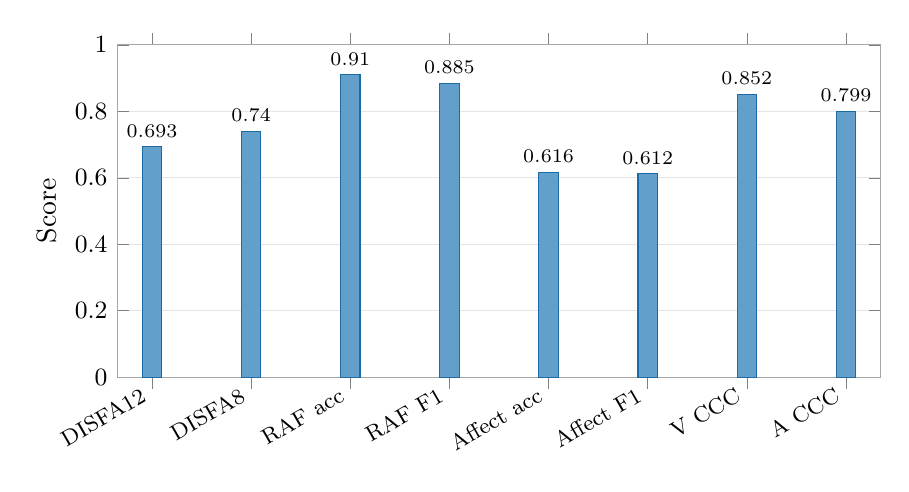
\begin{tikzpicture}
\begin{axis}[
  ybar,
  width=0.93\linewidth,
  height=58mm,
  ymin=0,
  ymax=1.0,
  ylabel={Score},
  symbolic x coords={DISFA12,DISFA8,RAF acc,RAF F1,Affect acc,Affect F1,V CCC,A CCC},
  xtick=data,
  x tick label style={rotate=30,anchor=east,font=\footnotesize},
  nodes near coords,
  nodes near coords style={font=\scriptsize, /pgf/number format/fixed, /pgf/number format/precision=3},
  bar width=7pt,
  enlarge x limits=0.05,
  ylabel near ticks,
  tick label style={font=\small},
  ymajorgrids=true,
  grid style={draw=black!10},
  axis line style={draw=black!35}
]
\addplot[fill=osblue!70,draw=osblue!90!black] coordinates {
  (DISFA12,0.693) (DISFA8,0.740) (RAF acc,0.910) (RAF F1,0.885)
  (Affect acc,0.616) (Affect F1,0.612) (V CCC,0.852) (A CCC,0.799)
};
\end{axis}
\end{tikzpicture}
\caption{공개 모델 카드의 높을수록 좋은 task-level 성능 지표. 서로 다른 지표(F1, accuracy, CCC)를 같은 축에 배치했으므로, 이 그림은 과제 간 우열 비교가 아니라 성능 범위의 요약으로 해석해야 한다.}
\label{fig:modelcard-bars}
\end{figure}

\begin{figure}[t]
\centering
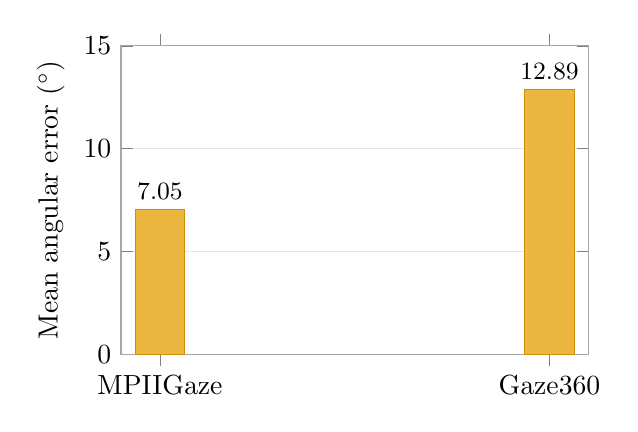
\begin{tikzpicture}
\begin{axis}[
  ybar,
  width=0.62\linewidth,
  height=55mm,
  ymin=0,
  ymax=15,
  ylabel={Mean angular error ($^\circ$)},
  symbolic x coords={MPIIGaze,Gaze360},
  xtick=data,
  nodes near coords,
  nodes near coords style={font=\small, /pgf/number format/fixed, /pgf/number format/precision=2},
  bar width=18pt,
  ymajorgrids=true,
  grid style={draw=black!10},
  axis line style={draw=black!35}
]
\addplot[fill=osorange!75,draw=osorange!90!black] coordinates {(MPIIGaze,7.05) (Gaze360,12.89)};
\end{axis}
\end{tikzpicture}
\caption{공개 모델 카드에 보고된 gaze estimation 평균 각도 오차. MPIIGaze는 leave-subject-out 설정이고, Gaze360은 held-out split 설정이다. 낮을수록 좋다.}
\label{fig:gaze-error}
\end{figure}

속도 벤치마크는 모델 처리량이 하드웨어 가속과 batch size에 크게 의존함을 보여준다. Apple M5 Max MPS 환경에서 \detector{}는 72프레임 short video 기준 batch 1에서 32.5 FPS, batch 4에서 93.5 FPS, batch 16에서 134.3 FPS를 기록하였다. 472프레임 long video에서는 각각 30.1 FPS, 86.7 FPS, 128.5 FPS를 기록하였다. 반면 CPU 환경에서는 short video와 long video 모두 batch size와 무관하게 약 2.0에서 2.4 FPS 범위에 머물렀다.

\begin{table}[t]
\centering
\caption{Py-Feat speed-clean-m5max 벤치마크와 현재 웹 데모 측정치. 모델 처리량은 warmup 이후 timed call이며, 웹 E2E는 카메라와 브라우저 렌더링을 포함한다.}
\label{tab:speed}
\small
\begin{tabularx}{\linewidth}{lXlccc}
\toprule
계층 & 환경 & 입력 & Batch & FPS & 지연/프레임 \\
\midrule
모델 처리량 & M5 Max MPS & 72 frames & 1 & 32.5 & 30.8 ms/frame \\
모델 처리량 & M5 Max MPS & 72 frames & 4 & 93.5 & 10.7 ms/frame \\
모델 처리량 & M5 Max MPS & 72 frames & 16 & 134.3 & 7.4 ms/frame \\
모델 처리량 & M5 Max MPS & 472 frames & 1 & 30.1 & 33.2 ms/frame \\
모델 처리량 & M5 Max MPS & 472 frames & 4 & 86.7 & 11.5 ms/frame \\
모델 처리량 & M5 Max MPS & 472 frames & 16 & 128.5 & 7.8 ms/frame \\
모델 처리량 & CPU & 72 frames & 1/4/16 & 2.3/2.4/2.0 & timed-call 기준 \\
모델 처리량 & CPU & 472 frames & 1/4/16 & 2.3/2.4/2.0 & timed-call 기준 \\
웹 E2E & Brave Browser & webcam demo & N/A & 22.1 & 45 ms latency \\
\bottomrule
\end{tabularx}
\end{table}

\begin{figure}[t]
\centering
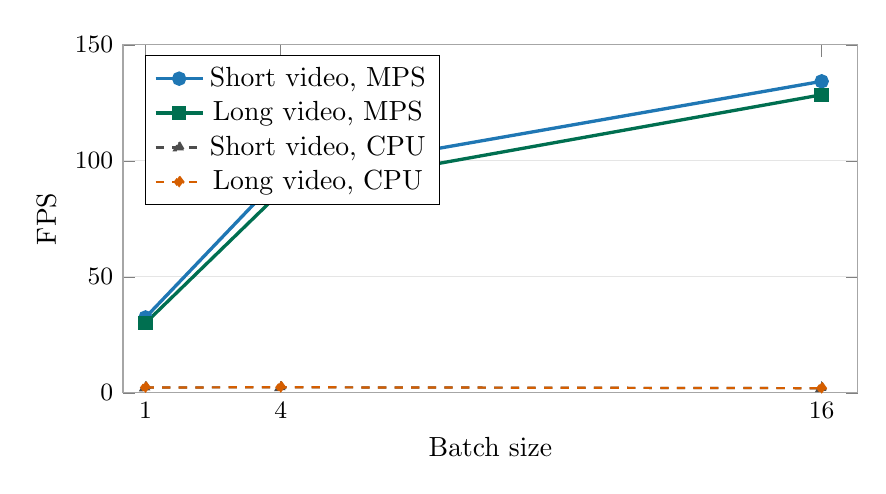
\begin{tikzpicture}
\begin{axis}[
  width=0.90\linewidth,
  height=60mm,
  xlabel={Batch size},
  ylabel={FPS},
  xmin=0.5,
  xmax=16.8,
  ymin=0,
  ymax=150,
  xtick={1,4,16},
  legend pos=north west,
  ymajorgrids=true,
  grid style={draw=black!10},
  axis line style={draw=black!35},
  tick label style={font=\small}
]
\addplot[color=osblue,mark=*,very thick] coordinates {(1,32.5) (4,93.5) (16,134.3)};
\addlegendentry{Short video, MPS}
\addplot[color=osgreen!70!black,mark=square*,very thick] coordinates {(1,30.1) (4,86.7) (16,128.5)};
\addlegendentry{Long video, MPS}
\addplot[color=osgray,mark=triangle*,thick,dashed] coordinates {(1,2.3) (4,2.4) (16,2.0)};
\addlegendentry{Short video, CPU}
\addplot[color=osred,mark=diamond*,thick,dashed] coordinates {(1,2.3) (4,2.4) (16,2.0)};
\addlegendentry{Long video, CPU}
\end{axis}
\end{tikzpicture}
\caption{Py-Feat speed-clean-m5max 벤치마크에서 \detector{}의 처리량 변화. MPS에서는 batch size 증가에 따라 처리량이 크게 증가하지만, CPU에서는 약 2 FPS 수준에 머문다.}
\label{fig:throughput}
\end{figure}

현재 웹 시연 문서에 기록된 Brave Browser capture 기준 엔드투엔드 성능은 약 22.1 FPS와 45 ms latency이다. 이 값은 모델의 순수 추론 처리량이 아니라 카메라 캡처, JPEG 전송, API 처리, 브라우저 canvas 렌더링을 포함한 사용자 관측 표시 성능이다. 따라서 MPS batch 16에서 보고된 128.5 또는 134.3 FPS와 웹 데모의 22.1 FPS는 직접 비교 대상이 아니다.

\begin{figure}[t]
\centering
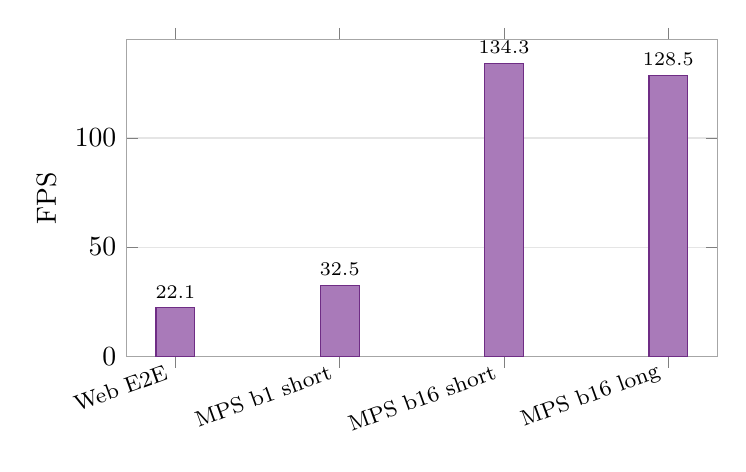
\begin{tikzpicture}
\begin{axis}[
  ybar,
  width=0.75\linewidth,
  height=56mm,
  ymin=0,
  ymax=145,
  ylabel={FPS},
  symbolic x coords={Web E2E,MPS b1 short,MPS b16 short,MPS b16 long},
  xtick=data,
  x tick label style={rotate=20,anchor=east,font=\footnotesize},
  nodes near coords,
  nodes near coords style={font=\scriptsize, /pgf/number format/fixed, /pgf/number format/precision=1},
  bar width=14pt,
  ymajorgrids=true,
  grid style={draw=black!10},
  axis line style={draw=black!35}
]
\addplot[fill=ospurple!65,draw=ospurple!90!black] coordinates {
  (Web E2E,22.1) (MPS b1 short,32.5) (MPS b16 short,134.3) (MPS b16 long,128.5)
};
\end{axis}
\end{tikzpicture}
\caption{웹 엔드투엔드 표시 성능과 모델 처리량 수치의 계층 차이. 같은 FPS 단위를 사용하지만, 웹 E2E는 capture-transfer-API-rendering까지 포함하므로 모델 timed-call 처리량과 동등한 벤치마크가 아니다.}
\label{fig:e2e-vs-model}
\end{figure}

\section{논의 및 한계}

본 연구의 핵심은 \detector{} 기반 웹 데모의 성능을 단일 숫자로 단순화하지 않고, 모델 정확도, 모델 처리량, 웹 엔드투엔드 표시 성능으로 분리하여 해석한 점이다. 공개 모델 카드 수치는 각 벤치마크 데이터셋에서의 과제별 일반화 성능을 나타내며, speed-clean-m5max 벤치마크는 특정 하드웨어와 batch 설정에서의 모델 처리량을 나타낸다. 반면 웹 데모의 FPS와 latency는 실제 사용자가 체감하는 표시 성능에 가까우며, 브라우저와 입출력 파이프라인의 비용을 포함한다.

가장 중요한 한계는 현재 저장소에 원자료와 평가 output이 포함되어 있지 않다는 점이다. 저장소에는 AFLFP 68-point landmark NME와 DISFA AU macro-F1/ICC 검증을 위한 deterministic pilot 코드가 구현되어 있으나, 본 논문에서는 해당 스크립트의 재실행 결과를 새로운 수치로 보고하지 않는다. 따라서 AFLFP NME, DISFA ICC, confidence interval, p-value, ablation 결과는 현재 단계에서 결과가 아니라 향후 작업으로 남겨야 한다.

두 번째 한계는 공개 모델 카드의 수치가 배포 체크포인트와 데이터셋별 protocol에 의존한다는 점이다. 본 논문은 모델 카드에 명시된 held-out/file-verified 수치를 인용하지만, 동일한 원자료, 체크포인트 hash, 패키지 버전, preprocessing을 고정하여 재실행한 독립 검증은 아직 수행하지 않았다. 실시간 데모의 웹 E2E 측정 역시 Brave Browser 캡처 기준 단일 관측값이므로, seed variance 또는 반복 측정 분산을 제공하지 못한다.

향후 연구에서는 원자료 접근 절차, 고정된 체크포인트 해시, 실행 환경 파일, deterministic seed, 평가 산출물 저장소를 함께 제공하여 전체 벤치마크를 재실행 가능하게 만들어야 한다. 또한 웹 데모 성능을 개선하려면 모델 추론 시간뿐 아니라 카메라 캡처, 프레임 인코딩, API 전송, canvas 렌더링의 단계별 profiling이 필요하다.

\section{재현성 정보}

\begin{sloppypar}
본 초안은 실제로 확인된 문서와 웹 출처의 수치만 사용했다. 공개 task-level 성능은 Hugging Face \model{} 모델 카드에서 확인했으며, 처리량 수치는 Py-Feat speed-clean-m5max benchmark 원문에서 확인했다. 웹 E2E 수치는 저장소의 주간 작업일지에 기록된 Brave Browser 캡처 측정값이다. 저장소 내 평가 관련 코드 경로는 \path{lib/py-feat-demo/benchmark_datasets.py}, \path{lib/py-feat-demo/pyfeat_benchmark_runner.py}, \path{lib/py-feat-demo/pyfeat_benchmark_disfa_runner.py}, \path{lib/py-feat-demo/pyfeat_benchmark_metrics.py}이다. 새로운 benchmark run, confidence interval, statistical test, ablation은 수행하지 않았으며, 따라서 본문에도 보고하지 않았다.
\end{sloppypar}

\section{결론}

Py-Feat \detector{} 기반 웹 데모는 단일 multi-task 모델을 통해 실시간 얼굴 행동 분석에 필요한 여러 출력을 통합적으로 제공한다. 공개 벤치마크는 AU, emotion, valence/arousal, gaze 과제에서 배포 체크포인트의 정량 성능을 보여주며, Apple M5 Max MPS 속도 벤치마크는 batch 처리 시 100 FPS 이상의 모델 처리량이 가능함을 보여준다. 동시에 웹 데모의 22.1 FPS와 45 ms latency는 모델 추론 외의 시스템 비용이 실제 사용자 경험에 중요한 영향을 미친다는 점을 드러낸다. 따라서 향후 보고서는 공개 성능, 모델 처리량, 웹 E2E 성능을 분리해 제시하고, 원자료 기반 재실행 결과가 확보될 때 AFLFP와 DISFA pilot 수치를 추가하는 방향으로 확장되어야 한다.

\bibliographystyle{plainnat}
\bibliography{references}

\end{document}
